%!TEX root = main.tex

\subsection{\textbf{RQ1:} What processes do software developers utilize for merge conflicts?}\label{RQ1}

\boldif{Results from interviews indicated that a common model of operating with merge conflicts exists.}
To understand the processes of software developers when collaboratively working on code, we asked interview participants to describe their current processes for handling merge conflicts.

\boldif{\textit{Add anecdotal quotes and descriptions from interviews to highlight these observations.}}
Several participants describe using tools that alert them to potential or current merge conflicts, processes for analyzing and understanding conflicting code prior to implementing a resolution, and the use of tools and checklists for validating that their resolution worked.
In the interview, P3 describes this process as:
\begin{quoting}
\textit{``Part of my job on the integration team requires that I check for bad regressions. I use scripts to track patches as they're being backported, so I know when and where to look if it introduces a conflict. And once I've fixed it, I try to compare with the previous version to make sure it works in a similar way.''}
\end{quoting}

\boldif{Based on these anecdotal observations, we construct an initial model of the processes that developers employ when working with merge conflicts, see Fig.~\ref{model}.}
Based on the initial anecdotal observations obtained from the interviews, we construct an initial model of the process developers experience between the introduction and resolution of merge conflicts.
Figure~\ref{model} provides an illustration of the model.
It consists of three phases: \emph{awareness, planning,} and \emph{evaluation}.

\begin{figure}[!htbp]
\centering
\fbox{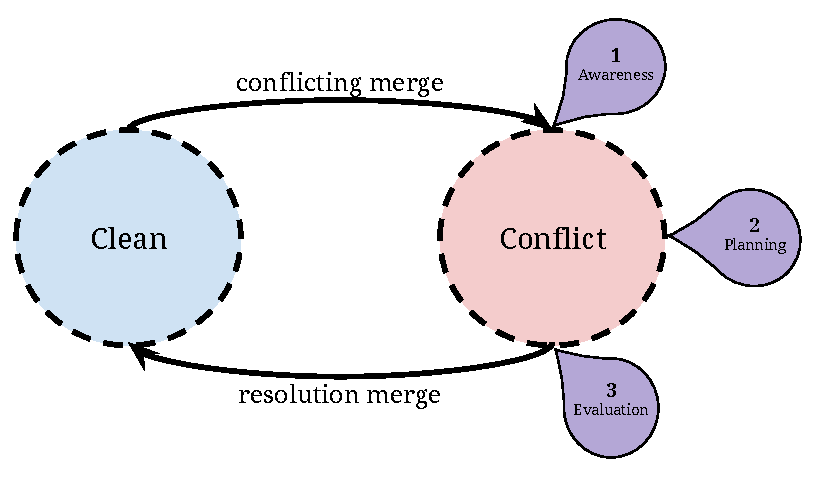
\includegraphics[width=0.98\textwidth,keepaspectratio]{imgs/MergeConflictModel}}
\caption{Model of Developer Processes for Merge Conflicts. Developers alternate between \textit{clean} and \textit{conflicting} states within their codebase. Developers maintain \textit{awareness}~(1) of conflicts within the codebase in different ways. Once aware, developers \textit{plan}~(2) a solution to fix the conflict. And finally, developers \textit{evaluate}~(3) the effectiveness of their deployed resolutions.}
\label{model}
\end{figure}

\boldif{Awareness is how developers become aware}
The \emph{awareness} phase consists of the actions developers take to become aware of merge conflicts.
This could be accidental, or passive, as the developer will become aware of a merge conflict when attempting to merge changes or perform a pull.
At the other end of the spectrum are developers who \emph{proactively} monitor for merge conflicts as they write code.
They are actively looking for changes that might be problematic, either manually or through the use of specialized tools.

\boldif{Planning is when developers plan their future actions}
Second, the \emph{planning} phase occurs after the developer has become aware that a conflict has occurred, and they are about to tackle the conflict.
Some developers might try and solve it immediately, while others might postpone the resolution.
Some might change their strategy depending on the conflict, incoming deadlines, etc.

\boldif{Evaluation is how developers check that their solution is correct}
Finally, after the conflict has been resolved, developers enter in the \emph{evaluation} phase.
In this phase, the developer has to evaluate their resolution before considering the conflict as resolved.
This is to ensure the correctness of the resultant code.
Possible actions during this stage are compilation and building the product at one end.
Developer wanting more guarantees can go a step further and run the tests.
Finally, some groups might have policies such as code reviews that need to be performed on the merge conflict resolution.
 
\boldif{To explore and validate this model, we asked developers to reflect upon how they become aware of merge conflicts, how they plan for merge conflict resolutions, and how they evaluate their resolutions in the \textit{Processes Survey}~(S1).}
In order to explore and validate this model, and our assumptions, we conducted the \emph{Processes Survey}~(S1).
We plan on understanding how developers become aware of a merge conflicts (what steps they take, what tools they use, etc.)
We also want to investigate their strategies for dealing with merge conflicts and how they decide whether the resolution has addressed all of their concerns.

\boldif{We present the results to these research questions in Section~\ref{RQ1a}, \ref{RQ1b}, and \ref{RQ1c}.}
Sections~\ref{RQ1a}, \ref{RQ1b}, and \ref{RQ1c} presents the results to these research questions.

\subsection{\textbf{RQ1a:} How do software developers become aware of merge conflicts?}\label{RQ1a}
\vspace*{-0.5\baselineskip}
\begin{quoting}
\textit{``It isn’t that they cannot find the solution. It is that they cannot see the problem.'' -- G.K. Chesterton}
\end{quoting}
\vspace*{+0.3\baselineskip}

\begin{table}[!htbp]
\renewcommand{\arraystretch}{1.3}
\caption{Merge Awareness Toolsets (Top 10) from Processes Survey (S1)}
\label{s1_toolset}
\centering
\begin{tabularx}{\textwidth}{ll|c}
\toprule
  \parnoteclear % tabularx will otherwise add each note thrice
  Tool & Description & \# Participants (\%)\parnote{Survey participants were allowed to provide multiple tools. Each entry represents the number (and percentage) of participants that responded with that particular tool. 57 out of 102 respondents (56\%) indicated the use of at least one merge awareness tool.}\\
\midrule
  Git & Version Control System & 32 (25.40\%)\\
  Email (unspecified) & Email Client or System & 7 (5.56\%)\\
  GitHub & Website & 7 (5.56\%)\\
  SVN & Version Control System & 4 (3.17\%)\\
  Visual Studio & IDE & 4 (3.17\%)\\
  PagerDuty & IT Incident Response Platform & 3 (2.38\%)\\
  GitLab & Website & 3 (2.38\%)\\
  Jenkins & Continuous Integration Platform & 3 (2.38\%)\\
  Team Foundation Server & Version Control System & 3 (2.38\%)\\
  VCS (unspecified) & Version Control System & 3 (2.38\%)\\
\bottomrule
\end{tabularx}
\parnotes
\end{table}

We asked Processes Survey (S1) participants to categorize and describe their monitoring processes: whether and how they monitor for merge conflicts, and how they determine the urgency of any merge conflicts that occur.
We found that 32.26\% of participants do not monitor for merge conflicts during their development sessions.
For the 67.74\% participants that indicate \textit{yes} or \textit{sometimes} to the question of monitoring for merge conflicts, we asked them to describe the processes and tools that they use for monitoring.

We identified 61 different tools from the 126 instances.
Some mentioned generic responses such as \textit{``email''}, for which we create a separate category.
Table~\ref{s1_toolset} lists the top 10 most common tools used by participants to monitor for merge conflicts.

In examining the list of these tools, we note that developers most often use version control systems (e.g. Git, SVN, TFS, and unspecified VCS) to handle tracking changes, and potentially identifying merge conflicts, within a codebase.
In this list, there is also one continuous integration (CI) platform (Jenkins), an IT incident response platform (PagerDuty), and two VCS-hosting websites (GitHub and GitLab).
This indicates that developers are currently relying on reactive tools that indicate the presence of merge conflicts after they have been introduced to a codebase.

We then evaluate responses for processes that are proactive or reactive in nature (using card sorting and negotiated agreement).
We find that 42 of 57 responses (73.68\%) described reactive processes of merge conflict monitoring; such as waiting for build systems notifications, examining commit logs, or checking code consistency during branch integration.

Examining the tools used by respondents with reactive processes, we find that they primarily use version control systems (Git, SVN, TFS, CVS) or continuous integration systems (Jenkins, Travis CI, TeamCity); 64.28\% and 29.19\% of respondents, respectively.
We find that developers are currently not leveraging the functionalities provided by many research prototypes (e.g., Palantir~\cite{palantir}, Crystal~\cite{Brun2011}) that are specifically designed to facilitate proactive conflict detection.

\boldif{Provide further discussion on the results; analysis between Caius and Nick still needed to group the processes into groups}

In addition, we identified \textbf{X} distinct categories of processes that developers use to monitor for merge conflicts (see Table~\ref{s1_monitoring_processes}).
 
\subsection{\textbf{RQ1b:} How do software developers plan for merge conflict resolutions?}\label{RQ1b}
\vspace*{-0.5\baselineskip}
\begin{quoting}
\textit{``If you are unable to understand the cause of a problem, it is impossible to solve it.'' –- Naoto Kan}
\end{quoting}
\vspace*{+0.3\baselineskip}

\subsection{\textbf{RQ1c:} How do software developers evaluate merge conflict resolutions?}\label{RQ1c}
\vspace*{-0.5\baselineskip}
\begin{quoting}
\textit{``We fail more often because we solve the wrong problem than because we get the wrong solution to the right problem.'' –- Russell L. Ackoff}
\end{quoting}
\vspace*{+0.3\baselineskip}

